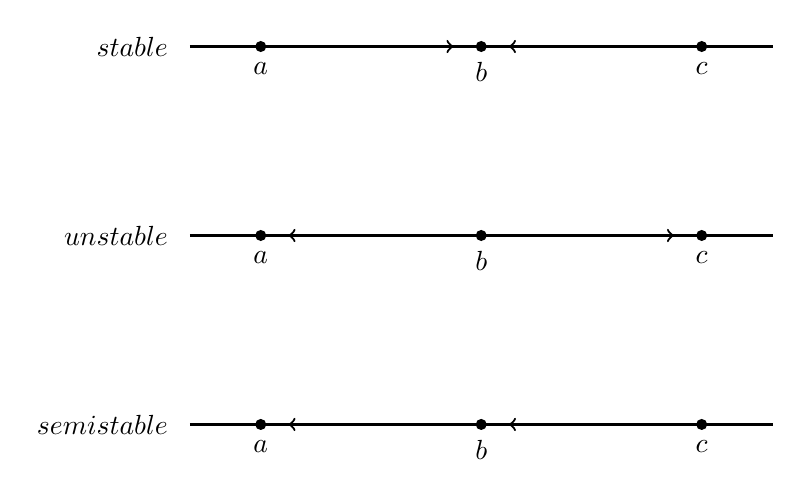
\begin{tikzpicture}[x=1cm,y=1cm,thick]
  % The three rows show the two intervals adjacent to b.
  \foreach \y/\case in {2.4/stable,0/unstable,-2.4/semistable} {
    \draw (-3.7,\y)--(3.7,\y);
    \foreach \x/\lab in {-2.8/a,0/b,2.8/c} {
      \fill (\x,\y) circle (2pt);
      \node[below=2pt] at (\x,\y) {$\lab$};
    }
    \node[left] at (-3.85,\y) {$\case$};
  }
  % Stable: both neighboring intervals flow toward b.
  \draw[->] (-2.45,2.4)--(-0.35,2.4);
  \draw[->] (2.45,2.4)--(0.35,2.4);
  % Unstable: both intervals flow away from b.
  \draw[<-] (-2.45,0)--(-0.35,0);
  \draw[->] (0.35,0)--(2.45,0);
  % Semistable: the left side leaves b while the right side approaches it.
  \draw[<-] (-2.45,-2.4)--(-0.35,-2.4);
  \draw[->] (2.45,-2.4)--(0.35,-2.4);
\end{tikzpicture}
